\documentclass[11pt,a4paper,notitlepage]{report}
% Shared preamble for the raw chapter-4 write-ups under docs/report/insights/.
%
% Each experiment_N/experiment_N.tex is a standalone, compilable LaTeX report
% written BEFORE anything goes into final_report/chapters/chapter_4_*.tex.
% It uses the final report's fonts, units and macros so that passages, tables
% and figures lift into the chapter without reformatting.
%
%   \documentclass[11pt,a4paper]{report}
%   % Shared preamble for the raw chapter-4 write-ups under docs/report/insights/.
%
% Each experiment_N/experiment_N.tex is a standalone, compilable LaTeX report
% written BEFORE anything goes into final_report/chapters/chapter_4_*.tex.
% It uses the final report's fonts, units and macros so that passages, tables
% and figures lift into the chapter without reformatting.
%
%   \documentclass[11pt,a4paper]{report}
%   % Shared preamble for the raw chapter-4 write-ups under docs/report/insights/.
%
% Each experiment_N/experiment_N.tex is a standalone, compilable LaTeX report
% written BEFORE anything goes into final_report/chapters/chapter_4_*.tex.
% It uses the final report's fonts, units and macros so that passages, tables
% and figures lift into the chapter without reformatting.
%
%   \documentclass[11pt,a4paper]{report}
%   \input{../common/preamble}
%   \begin{document} ...
%
% Figures and tables are NOT copied: \graphicspath and \reporttable resolve into
% final_report/figures/ and final_report/tables/, so the raw write-up always
% shows the same artefacts as the chapter.  Compile with:  latexmk -pdf <file>

\usepackage[T1]{fontenc}
\usepackage[utf8]{inputenc}
\usepackage{mathptmx}
\usepackage[scaled=0.92]{helvet}
\usepackage{courier}
\usepackage[a4paper,left=30mm,right=20mm,top=25mm,bottom=25mm]{geometry}
\usepackage{microtype}
\usepackage{booktabs}
\usepackage{tabularx}
\usepackage{longtable}
\usepackage{array}
\usepackage{multirow}
\usepackage{amsmath}
\usepackage{amssymb}
\usepackage{ifthen}
\usepackage{siunitx}
\usepackage{graphicx}
\usepackage{placeins}
\usepackage{caption}
\usepackage{enumitem}
\usepackage[table]{xcolor}
\usepackage{rotating}
\PassOptionsToPackage{hyphens}{url}\usepackage{url}
\usepackage[hidelinks]{hyperref}
\usepackage[nameinlink,noabbrev]{cleveref}

\graphicspath{{../../final_report/}{../../final_report/figures/}}
% \reporttable{name} inputs final_report/tables/name.tex
\newcommand{\reporttable}[1]{\input{../../final_report/tables/#1}}

\newcommand{\repo}[1]{\texttt{\detokenize{#1}}}
\sisetup{detect-all,group-separator={,},range-phrase=--,range-units=single}
\DeclareSIUnit{\pixel}{px}
\DeclareSIUnit{\mebi}{Mi}
\captionsetup{font=small,labelfont=bf}
\setlist{nosep}
\setlength{\parskip}{4pt}
\setlength{\LTcapwidth}{\textwidth}

% ---- result-slot status (RENDERED here, unlike in the final report)
\definecolor{stcompleted}{HTML}{A5D6A7}
\definecolor{stpartial}{HTML}{FFF2CC}
\definecolor{stuntested}{HTML}{FFD8A8}
\definecolor{stblocked}{HTML}{FFCDD2}
\definecolor{stfailed}{HTML}{FFCDD2}
\definecolor{stplanned}{HTML}{E0E0E0}
\newcommand{\slotstatus}[2]{%
  \par\noindent\fcolorbox{black!40}{st#1}{\parbox{\dimexpr\textwidth-2\fboxsep-2\fboxrule}{%
    \textbf{Status: #1.}\ #2}}\par\medskip}
\newcommand{\status}[1]{\textbf{#1}}

% ---- queries: RENDERED in red here so a reader sees every open concern in place
\definecolor{flagred}{HTML}{B00000}
\newcommand{\flag}[1]{\textcolor{flagred}{#1}}
\newcommand{\moved}[1]{#1}
\newenvironment{queried}[1][Questionable]%
  {\par\addvspace{0.6ex}\begingroup\color{flagred}\noindent
   \textbf{[#1]}\ \ignorespaces}%
  {\par\endgroup\addvspace{0.6ex}}

% ---- per-block performance marks (section 4.5 diagrams)
\definecolor{perfgood}{HTML}{A5D6A7}
\definecolor{perfpoor}{HTML}{FFCDD2}
\definecolor{perfnoeffect}{HTML}{D9EAF7}
\definecolor{perfnone}{HTML}{FFF2CC}
\newcommand{\perfmark}[1]{%
  \ifthenelse{\equal{#1}{good}}{\colorbox{perfgood}{\scriptsize good}}{%
  \ifthenelse{\equal{#1}{poor}}{\colorbox{perfpoor}{\scriptsize poor}}{%
  \ifthenelse{\equal{#1}{noeffect}}{\colorbox{perfnoeffect}{\scriptsize no effect}}{%
  \colorbox{perfnone}{\scriptsize no claim}}}}}

%   \begin{document} ...
%
% Figures and tables are NOT copied: \graphicspath and \reporttable resolve into
% final_report/figures/ and final_report/tables/, so the raw write-up always
% shows the same artefacts as the chapter.  Compile with:  latexmk -pdf <file>

\usepackage[T1]{fontenc}
\usepackage[utf8]{inputenc}
\usepackage{mathptmx}
\usepackage[scaled=0.92]{helvet}
\usepackage{courier}
\usepackage[a4paper,left=30mm,right=20mm,top=25mm,bottom=25mm]{geometry}
\usepackage{microtype}
\usepackage{booktabs}
\usepackage{tabularx}
\usepackage{longtable}
\usepackage{array}
\usepackage{multirow}
\usepackage{amsmath}
\usepackage{amssymb}
\usepackage{ifthen}
\usepackage{siunitx}
\usepackage{graphicx}
\usepackage{placeins}
\usepackage{caption}
\usepackage{enumitem}
\usepackage[table]{xcolor}
\usepackage{rotating}
\PassOptionsToPackage{hyphens}{url}\usepackage{url}
\usepackage[hidelinks]{hyperref}
\usepackage[nameinlink,noabbrev]{cleveref}

\graphicspath{{../../final_report/}{../../final_report/figures/}}
% \reporttable{name} inputs final_report/tables/name.tex
\newcommand{\reporttable}[1]{\input{../../final_report/tables/#1}}

\newcommand{\repo}[1]{\texttt{\detokenize{#1}}}
\sisetup{detect-all,group-separator={,},range-phrase=--,range-units=single}
\DeclareSIUnit{\pixel}{px}
\DeclareSIUnit{\mebi}{Mi}
\captionsetup{font=small,labelfont=bf}
\setlist{nosep}
\setlength{\parskip}{4pt}
\setlength{\LTcapwidth}{\textwidth}

% ---- result-slot status (RENDERED here, unlike in the final report)
\definecolor{stcompleted}{HTML}{A5D6A7}
\definecolor{stpartial}{HTML}{FFF2CC}
\definecolor{stuntested}{HTML}{FFD8A8}
\definecolor{stblocked}{HTML}{FFCDD2}
\definecolor{stfailed}{HTML}{FFCDD2}
\definecolor{stplanned}{HTML}{E0E0E0}
\newcommand{\slotstatus}[2]{%
  \par\noindent\fcolorbox{black!40}{st#1}{\parbox{\dimexpr\textwidth-2\fboxsep-2\fboxrule}{%
    \textbf{Status: #1.}\ #2}}\par\medskip}
\newcommand{\status}[1]{\textbf{#1}}

% ---- queries: RENDERED in red here so a reader sees every open concern in place
\definecolor{flagred}{HTML}{B00000}
\newcommand{\flag}[1]{\textcolor{flagred}{#1}}
\newcommand{\moved}[1]{#1}
\newenvironment{queried}[1][Questionable]%
  {\par\addvspace{0.6ex}\begingroup\color{flagred}\noindent
   \textbf{[#1]}\ \ignorespaces}%
  {\par\endgroup\addvspace{0.6ex}}

% ---- per-block performance marks (section 4.5 diagrams)
\definecolor{perfgood}{HTML}{A5D6A7}
\definecolor{perfpoor}{HTML}{FFCDD2}
\definecolor{perfnoeffect}{HTML}{D9EAF7}
\definecolor{perfnone}{HTML}{FFF2CC}
\newcommand{\perfmark}[1]{%
  \ifthenelse{\equal{#1}{good}}{\colorbox{perfgood}{\scriptsize good}}{%
  \ifthenelse{\equal{#1}{poor}}{\colorbox{perfpoor}{\scriptsize poor}}{%
  \ifthenelse{\equal{#1}{noeffect}}{\colorbox{perfnoeffect}{\scriptsize no effect}}{%
  \colorbox{perfnone}{\scriptsize no claim}}}}}

%   \begin{document} ...
%
% Figures and tables are NOT copied: \graphicspath and \reporttable resolve into
% final_report/figures/ and final_report/tables/, so the raw write-up always
% shows the same artefacts as the chapter.  Compile with:  latexmk -pdf <file>

\usepackage[T1]{fontenc}
\usepackage[utf8]{inputenc}
\usepackage{mathptmx}
\usepackage[scaled=0.92]{helvet}
\usepackage{courier}
\usepackage[a4paper,left=30mm,right=20mm,top=25mm,bottom=25mm]{geometry}
\usepackage{microtype}
\usepackage{booktabs}
\usepackage{tabularx}
\usepackage{longtable}
\usepackage{array}
\usepackage{multirow}
\usepackage{amsmath}
\usepackage{amssymb}
\usepackage{ifthen}
\usepackage{siunitx}
\usepackage{graphicx}
\usepackage{placeins}
\usepackage{caption}
\usepackage{enumitem}
\usepackage[table]{xcolor}
\usepackage{rotating}
\PassOptionsToPackage{hyphens}{url}\usepackage{url}
\usepackage[hidelinks]{hyperref}
\usepackage[nameinlink,noabbrev]{cleveref}

\graphicspath{{../../final_report/}{../../final_report/figures/}}
% \reporttable{name} inputs final_report/tables/name.tex
\newcommand{\reporttable}[1]{\input{../../final_report/tables/#1}}

\newcommand{\repo}[1]{\texttt{\detokenize{#1}}}
\sisetup{detect-all,group-separator={,},range-phrase=--,range-units=single}
\DeclareSIUnit{\pixel}{px}
\DeclareSIUnit{\mebi}{Mi}
\captionsetup{font=small,labelfont=bf}
\setlist{nosep}
\setlength{\parskip}{4pt}
\setlength{\LTcapwidth}{\textwidth}

% ---- result-slot status (RENDERED here, unlike in the final report)
\definecolor{stcompleted}{HTML}{A5D6A7}
\definecolor{stpartial}{HTML}{FFF2CC}
\definecolor{stuntested}{HTML}{FFD8A8}
\definecolor{stblocked}{HTML}{FFCDD2}
\definecolor{stfailed}{HTML}{FFCDD2}
\definecolor{stplanned}{HTML}{E0E0E0}
\newcommand{\slotstatus}[2]{%
  \par\noindent\fcolorbox{black!40}{st#1}{\parbox{\dimexpr\textwidth-2\fboxsep-2\fboxrule}{%
    \textbf{Status: #1.}\ #2}}\par\medskip}
\newcommand{\status}[1]{\textbf{#1}}

% ---- queries: RENDERED in red here so a reader sees every open concern in place
\definecolor{flagred}{HTML}{B00000}
\newcommand{\flag}[1]{\textcolor{flagred}{#1}}
\newcommand{\moved}[1]{#1}
\newenvironment{queried}[1][Questionable]%
  {\par\addvspace{0.6ex}\begingroup\color{flagred}\noindent
   \textbf{[#1]}\ \ignorespaces}%
  {\par\endgroup\addvspace{0.6ex}}

% ---- per-block performance marks (section 4.5 diagrams)
\definecolor{perfgood}{HTML}{A5D6A7}
\definecolor{perfpoor}{HTML}{FFCDD2}
\definecolor{perfnoeffect}{HTML}{D9EAF7}
\definecolor{perfnone}{HTML}{FFF2CC}
\newcommand{\perfmark}[1]{%
  \ifthenelse{\equal{#1}{good}}{\colorbox{perfgood}{\scriptsize good}}{%
  \ifthenelse{\equal{#1}{poor}}{\colorbox{perfpoor}{\scriptsize poor}}{%
  \ifthenelse{\equal{#1}{noeffect}}{\colorbox{perfnoeffect}{\scriptsize no effect}}{%
  \colorbox{perfnone}{\scriptsize no claim}}}}}

\setcounter{chapter}{4}
\renewcommand{\thesection}{4.4.\arabic{section}}
\renewcommand{\thefigure}{4.\arabic{figure}}
\renewcommand{\thetable}{4.\arabic{table}}
\title{Experiment 4: Autonomous Navigation on the Reconstructed Map\\
       \large Raw write-up for Chapter 4, Section 4.4}
\author{Bolton Athit Davies}
\date{Reporting cutoff: 12 November 2026}
\begin{document}
\maketitle

\noindent\textbf{Purpose of this document.} This is the raw, complete write-up
of Experiment 4, written before the thesis chapter; Section 4.4 of the final
report is extracted from it. The experiment is \status{partial}. One of its two
questions now has data: how well the pose published on a prior map tracks
ground truth while the robot drives. The other --- whether the planner reaches
a goal set without colliding --- has none, and its reporting rules are left
exactly as they were fixed before any run existed.

% =====================================================================
\FloatBarrier
\section{Simulation}
\label{sec:exp4-sim}

\slotstatus{partial}{Seven live runs on 12 November 2026, in three of the four
worlds, measure the localisation against ground truth over hand-driven routes
of \SIrange{21}{153}{\metre}. No goal was commanded in any of them, so the
goal-reaching measures of the reporting rules below are still unused and that
half of the experiment remains \status{planned}. The protocol, goal set and
success criteria are now fixed in code (\repo{script/exp4_protocol.yaml},
generated by \repo{script/exp4_goals.py}), which is what the previous revision
of this document recorded as missing. Mechanisms are analysed separately in
\path{insights/experiment_4_insight/}.}

\paragraph{Objective.} Establish whether the map of the simulation slot of
Experiment~3 is good enough to navigate on: whether the robot can relocalise
against a prior it did not build, hold that pose while driving, plan a path
through the map, and reach a sequence of goals without colliding with structure
the map got wrong. Experiment~3 scores the map as geometry; this experiment
scores it as something a planner consumes. The two are not the same question,
and the false obstacles Experiment~3 reports are the reason: a map can be
\SI{80}{\percent} precise and still block the one aisle the robot needs.

\paragraph{Process.} \repo{vslam_navigation} exposes the three stages as
separate entry points, so the experiment follows them in order:
\texttt{mapping\_sim} builds the prior, \texttt{localize\_sim} gives a
read-only fix against it, and \texttt{navigate\_sim} adds the planner, the
localisation gate and the command interface. The prior is one of the databases
already scored in the simulation slot of Experiment~3, so that map quality and
navigation outcome are measured on the same artefact. The runs reported here
were driven by the operator rather than by the planner; \repo{exp4\_navigate.py}
provides both modes (\texttt{--drive} and \texttt{--run}) and records the same
data either way.

\paragraph{Datasets and configuration.} The two realistic worlds of the
methodology chapter and the closure-free priors built from their mapping
recordings: \repo{dataset_allsensor_realistic_map} (U, 148 nodes) and
\repo{dataset_allsensor_realistic_01_map} (I, 127 nodes). No bag is replayed:
the simulator is driven live, because a navigation outcome depends on the
control loop and cannot be reconstructed from a recording. Every run used the
configuration frozen in the protocol file: \repo{Vis/EstimationType}~0, which
requires matched feature positions to agree in metres rather than merely to
reproject, and a \SI{5}{\second} hold on the back end so that no correction can
be latched from the front end's unstable first second. Both settings come from
the acceptance sweep of 11--12 November and are recorded in each run's
\repo{outcome.json}.

\paragraph{Frames.} Ground truth is the Gazebo world frame; the prior, the
goals and the published pose are the map frame. The two are reconciled by a
closed-form planar fit of every graph node against the mapping run's ground
truth, which gives \SI{179.95}{\degree} and \SI{-179.61}{\degree} of rotation
for the U and I priors --- the map frame is the spawn, turned around --- with
median residuals of \SI{0.103}{\metre} and \SI{0.055}{\metre}. The ground truth
reports the model origin and every estimate reports the camera/IMU body, so the
\SI{0.338}{\metre} lever arm is applied to the ground truth before the fit and
before any comparison, and never to recorded data.
\flag{Two corrections belong on the record here.} First, an earlier revision
fitted the transform against uncorrected ground truth and reported the resulting
\SI{0.337}{\metre} residual as confirmation that the fit was right, on the
grounds that it equalled the lever arm. That was the bias, not the evidence: a
rigid transform cannot absorb an offset that rotates with the body, so it
absorbed part of it as translation and left the rest as residual. Applying the
lever arm before the fit drops the residual to \SI{0.103}{\metre} and
\SI{0.055}{\metre}.

Second, and larger, the same revision applied the lever arm to ground truth in
the \emph{comparison} as well, which was wrong and inflated every error this
slot reported by about a third of a metre. The recorder samples
\texttt{map}~$\rightarrow$~\texttt{base\_link}, and the published
\texttt{base\_link} sits where the model origin is, so ground truth needs no
correction to meet it. Decomposing the error along and across the direction of
travel is what exposed it: with the lever arm applied, the along-track mean was
\SIrange{-0.28}{-0.38}{\metre} in all seven runs while the cross-track mean sat
near zero --- a constant displacement in the direction of travel, of the lever
arm's length, in the same direction every time, and not scaling with speed, so
not a latency either. Without it the along-track mean is
\SIrange{-0.16}{+0.04}{\metre} and changes sign between runs. The medians fell
from \SIrange{0.36}{0.62}{\metre} to \SIrange{0.10}{0.36}{\metre}
accordingly. The lever arm still belongs in the alignment, which fits body-frame
node poses; the two are different quantities and their frames legitimately
differ.

\paragraph{Reporting rules, goal-reaching.} \flag{Fixed before any run exists,
so that the result cannot be chosen after the fact, and left unchanged here.} A
goal counts as reached when the base frame is within \SI{0.25}{\metre} and
\SI{10}{\degree} of it and the planner reports success. Per run the measures
are: the share of goals reached, the path length against the shortest
collision-free path in the ground-truth occupancy grid, the number of
collisions with true structure, the number of Nav2 recovery behaviours
triggered, the share of the run with a valid localisation fix, and the wall
time to complete the goal set. A run that loses localisation and does not
recover within \SI{30}{\second} is reported as failed, not excluded.

\paragraph{Reporting rules, pose tracking.} \flag{Defined after these data
existed, and reported as the weaker claim it is.} Error is the planar distance
between the published \texttt{map}~$\rightarrow$~\texttt{base\_link} transform,
sampled at \SI{2}{\hertz}, and the lever-arm-corrected ground truth
interpolated to the same instants. That transform is used rather than
\texttt{/localization\_pose} because it is what RViz draws and Nav2 consumes,
and it includes the front end's dead reckoning between accepted fixes. The
error is reported as a median, a 95th percentile, a maximum, the median over
each half of the run, and split into the length of the mean error vector
(offset) and the standard deviation about it (scatter). A pose step over
\SI{1}{\metre} between consecutive samples is counted as a jump, excluding the
seed transition and the acquisition snap. Every run is reported on its own, as
in the other slots.

\paragraph{Results.} \Cref{tab:exp4-tracking} gives the seven runs and
\cref{fig:exp4-normal,fig:exp4-ilayout,fig:exp4-offset,fig:exp4-diverged} draw four of them.
The pose tracks ground truth to a median of \SIrange{0.10}{0.36}{\metre},
with a median across runs of \SI{0.162}{\metre}, and the error is bounded
rather than growing: in six of the seven runs the median over the first and
second half of the run agree. Minimum ground-truth clearance to a static model
never fell below \SI{0.58}{\metre}, so no run collided.

\begin{table}[htbp]
\centering\small
\caption{Pose tracking against ground truth, 12 November 2026. Route shapes
were driven by hand: straight, approximately square, approximately a
figure-of-eight. ``Over 1\,m'' is the longest unbroken stretch with the error above a metre and
``ended'' the median over the last tenth of the run, i.e. whether it came back.
Offset and scatter, reported in the text, are \SIrange{0.07}{0.27}{\metre} and
\SIrange{0.04}{0.24}{\metre} respectively. Blind is the share of localisation poses carrying
RTAB-Map's no-information covariance. Ground truth is compared without a lever
arm, for the reason given under Frames.}
\label{tab:exp4-tracking}
\begin{tabular}{llrrrrrrrrr}
\toprule
World & Route & Driven & Dur. & Med. & p95 & Max & Over & Ended & Blind & Jumps \\
      &       & (m)    & (s)  & (m)  & (m) & (m) & 1\,m (s) & (m) & & \\
\midrule
U static  & straight &  24.6 &  25 & 0.162 & 0.226 &  0.24 &  0.0 & 0.033 & 0.045 & 0 \\
U static  & square   & 109.2 &  86 & 0.188 & 6.355 &  6.80 & 36.0 & 0.106 & 0.016 & 4 \\
U static  & figure-8 & 152.0 & 124 & 0.098 & 3.750 &  3.99 & 23.5 & 0.120 & 0.013 & 3 \\
I static  & straight &  20.9 &  25 & 0.097 & 0.598 &  0.61 &  0.0 & 0.084 & 0.158 & 1 \\
I static  & square   &  66.8 &  57 & 0.361 & 0.631 &  0.69 &  0.0 & 0.113 & 0.068 & 2 \\
I static  & figure-8 & 123.7 & 122 & 0.136 & 0.749 &  0.93 &  0.0 & 0.117 & 0.047 & 1 \\
U dynamic & straight &  26.0 &  30 & 0.298 & 1.077 &  1.17 &  2.5 & 0.066 & 0.103 & 1 \\
\bottomrule
\end{tabular}
\end{table}



\begin{figure}[p]
  \centering
  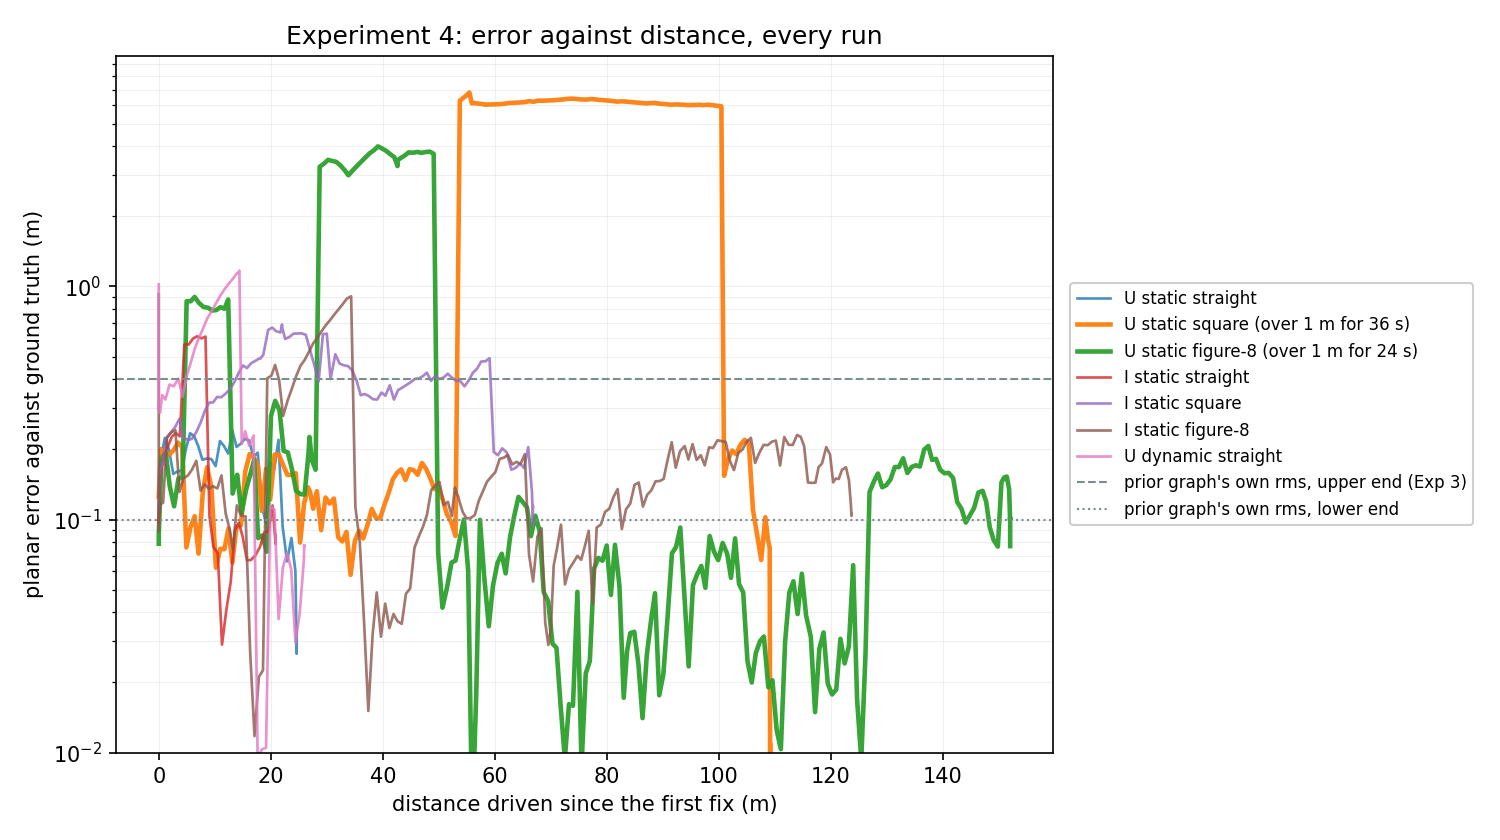
\includegraphics[width=\textwidth]{fig/exp4_error_vs_distance.png}
  \caption{Every run on one axis: planar error against distance driven since
  the first fix, logarithmic. Distance rather than time, so that runs driven at
  different speeds compare. The two grey lines are the rms accuracy Experiment~3
  measures for these priors' own graphs, \SIrange{0.10}{0.40}{\metre}: most of
  the time most runs sit between them, which is the bound this slot reports.
  The two shelves are the excursions of \cref{tab:exp4-tracking} --- flat, not
  ramped, so the pose steps to a wrong place and holds it rather than drifting
  away. Both end abruptly when a correct fix lands.}
  \label{fig:exp4-summary}
\end{figure}

\begin{figure}[p]
  \centering
  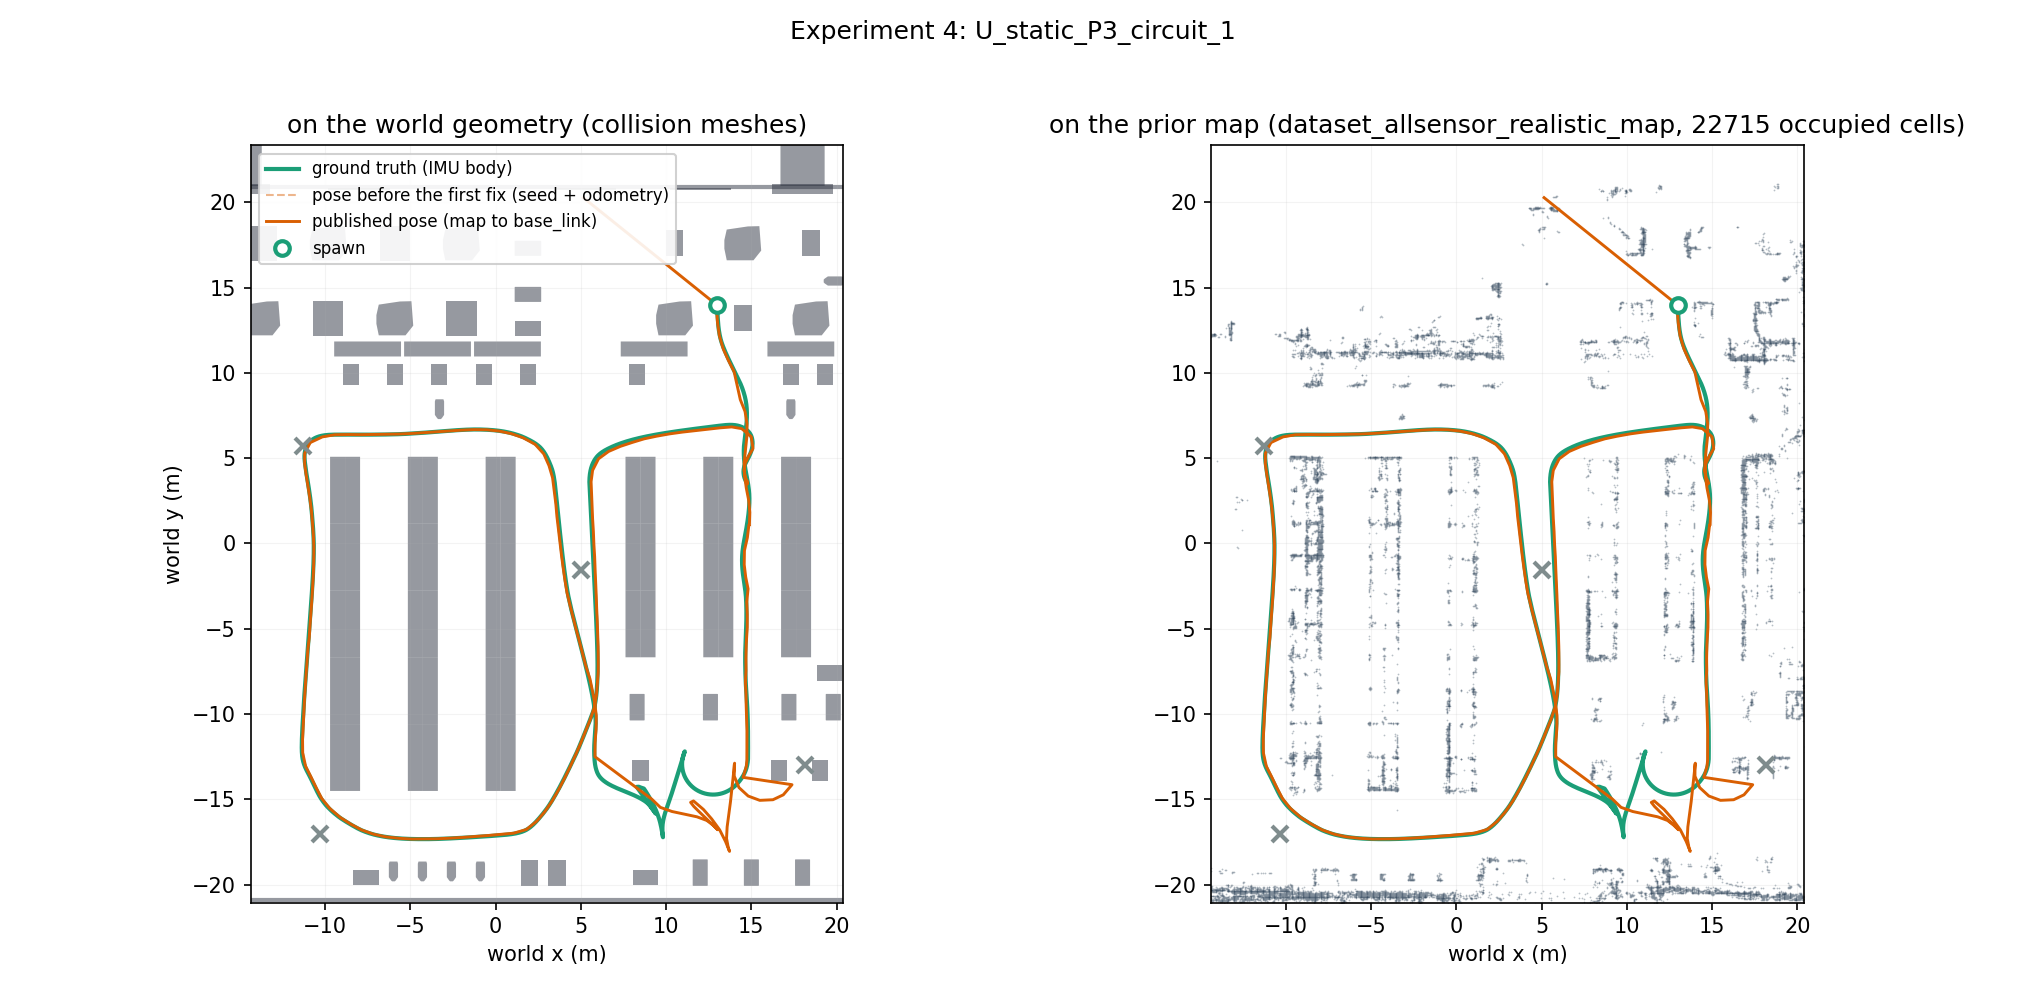
\includegraphics[width=\textwidth]{fig/exp4_path_U_static_P3_circuit_1.png}
  \caption{\texttt{U\_static}, figure-of-eight, \SI{152}{\metre}. Left: the
  published pose against ground truth on the world's collision-mesh footprints,
  the same underlay the chapter 3 scene figures use. Right: the same two tracks
  on the prior's exported occupancy grid, brought into the world frame by the
  fit of \cref{sec:exp4-sim}. The grid's shelf rows landing on the mesh
  footprints is the alignment confirming itself; the thick band at the right
  wall against the mesh's thin line is the wall displacement Experiment~3
  reports. The dashed segment is the pose before the first fix, which is the
  seed composed with raw odometry and is not a tracking error. Median error
  \SI{0.098}{\metre}.}
  \label{fig:exp4-normal}
\end{figure}


\begin{figure}[p]
  \centering
  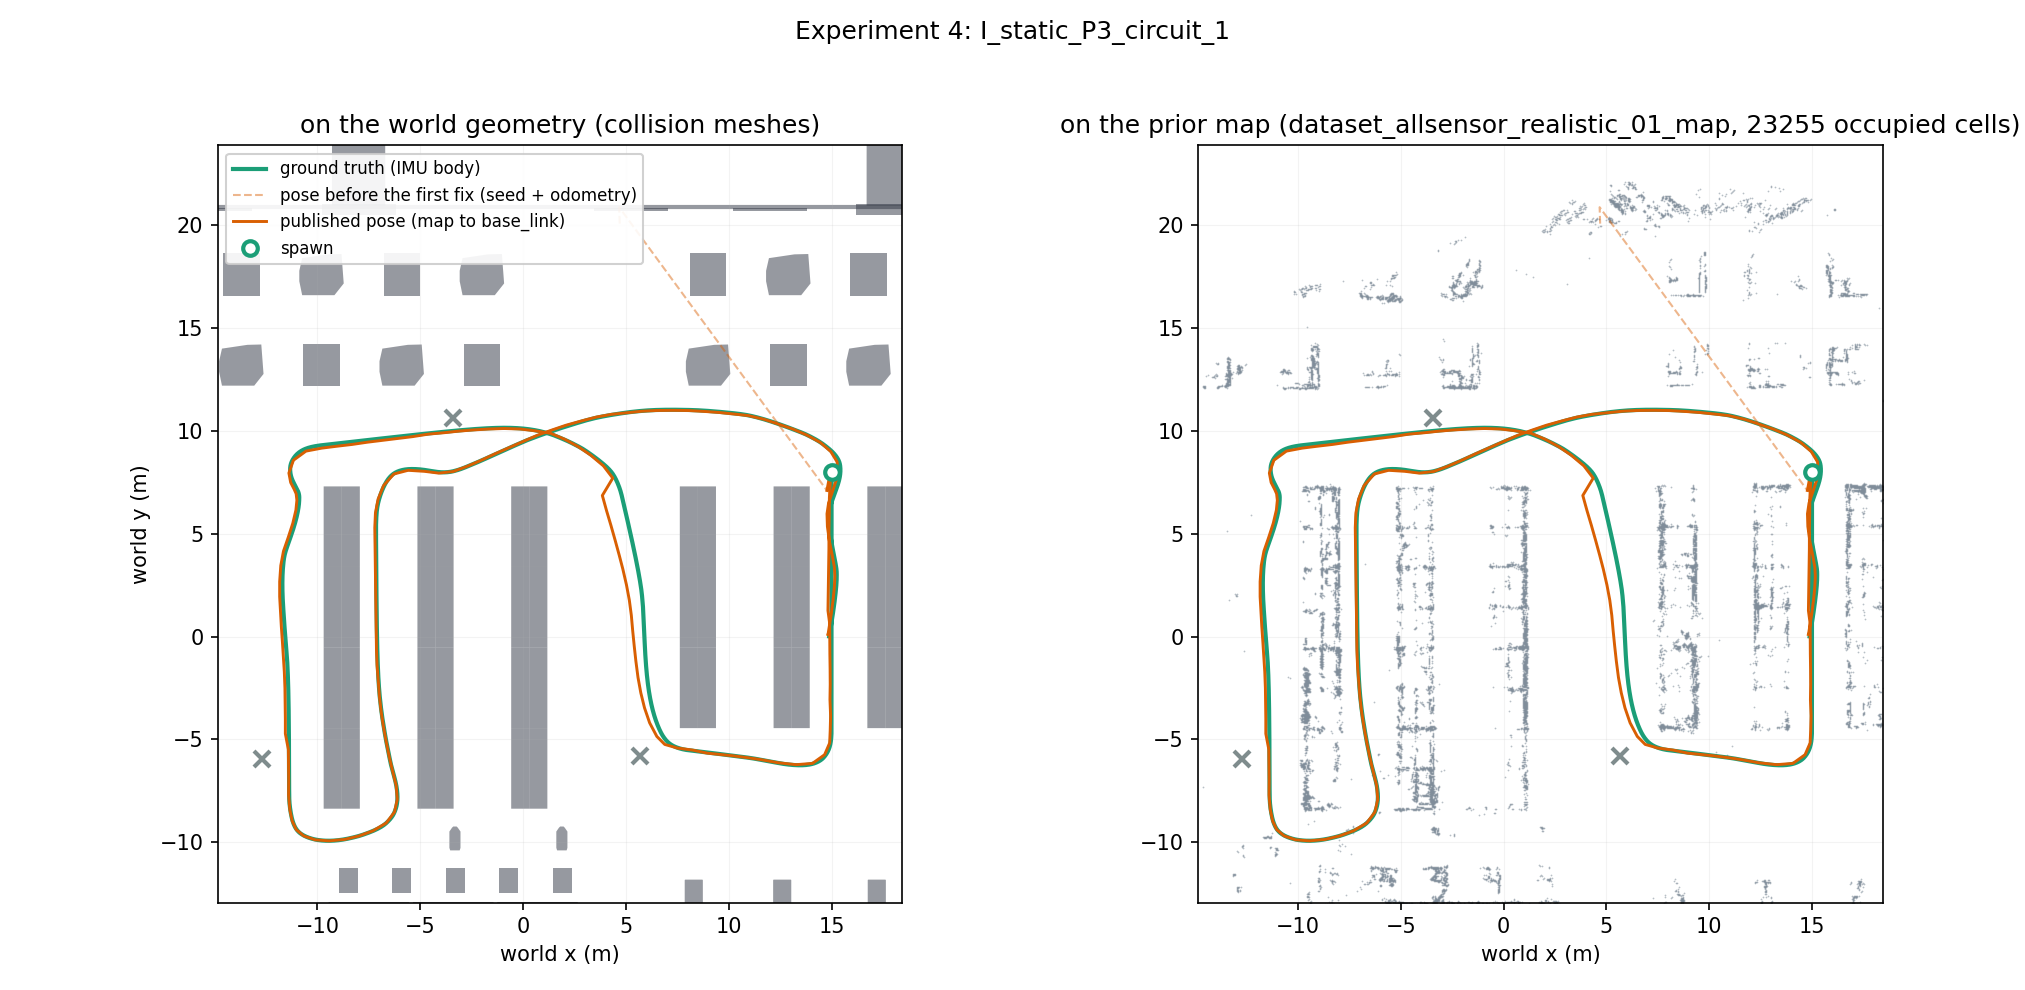
\includegraphics[width=\textwidth]{fig/exp4_path_I_static_P3_circuit_1.png}
  \caption{\texttt{I\_static}, figure-of-eight, \SI{124}{\metre}: the cleanest
  run of the seven, median \SI{0.136}{\metre} and maximum \SI{0.93}{\metre}, on
  the second layout and its own prior
  (\repo{dataset_allsensor_realistic_01_map}, 23\,255 occupied cells). The
  layouts differ in aisle arrangement, so this is not a repeat of
  \cref{fig:exp4-normal} in a different place: the route crosses its own path
  twice and the pose holds through both crossings, which is where a prior that
  aliases between aisles would show it. Conventions as \cref{fig:exp4-normal}.}
  \label{fig:exp4-ilayout}
\end{figure}

\begin{figure}[p]
  \centering
  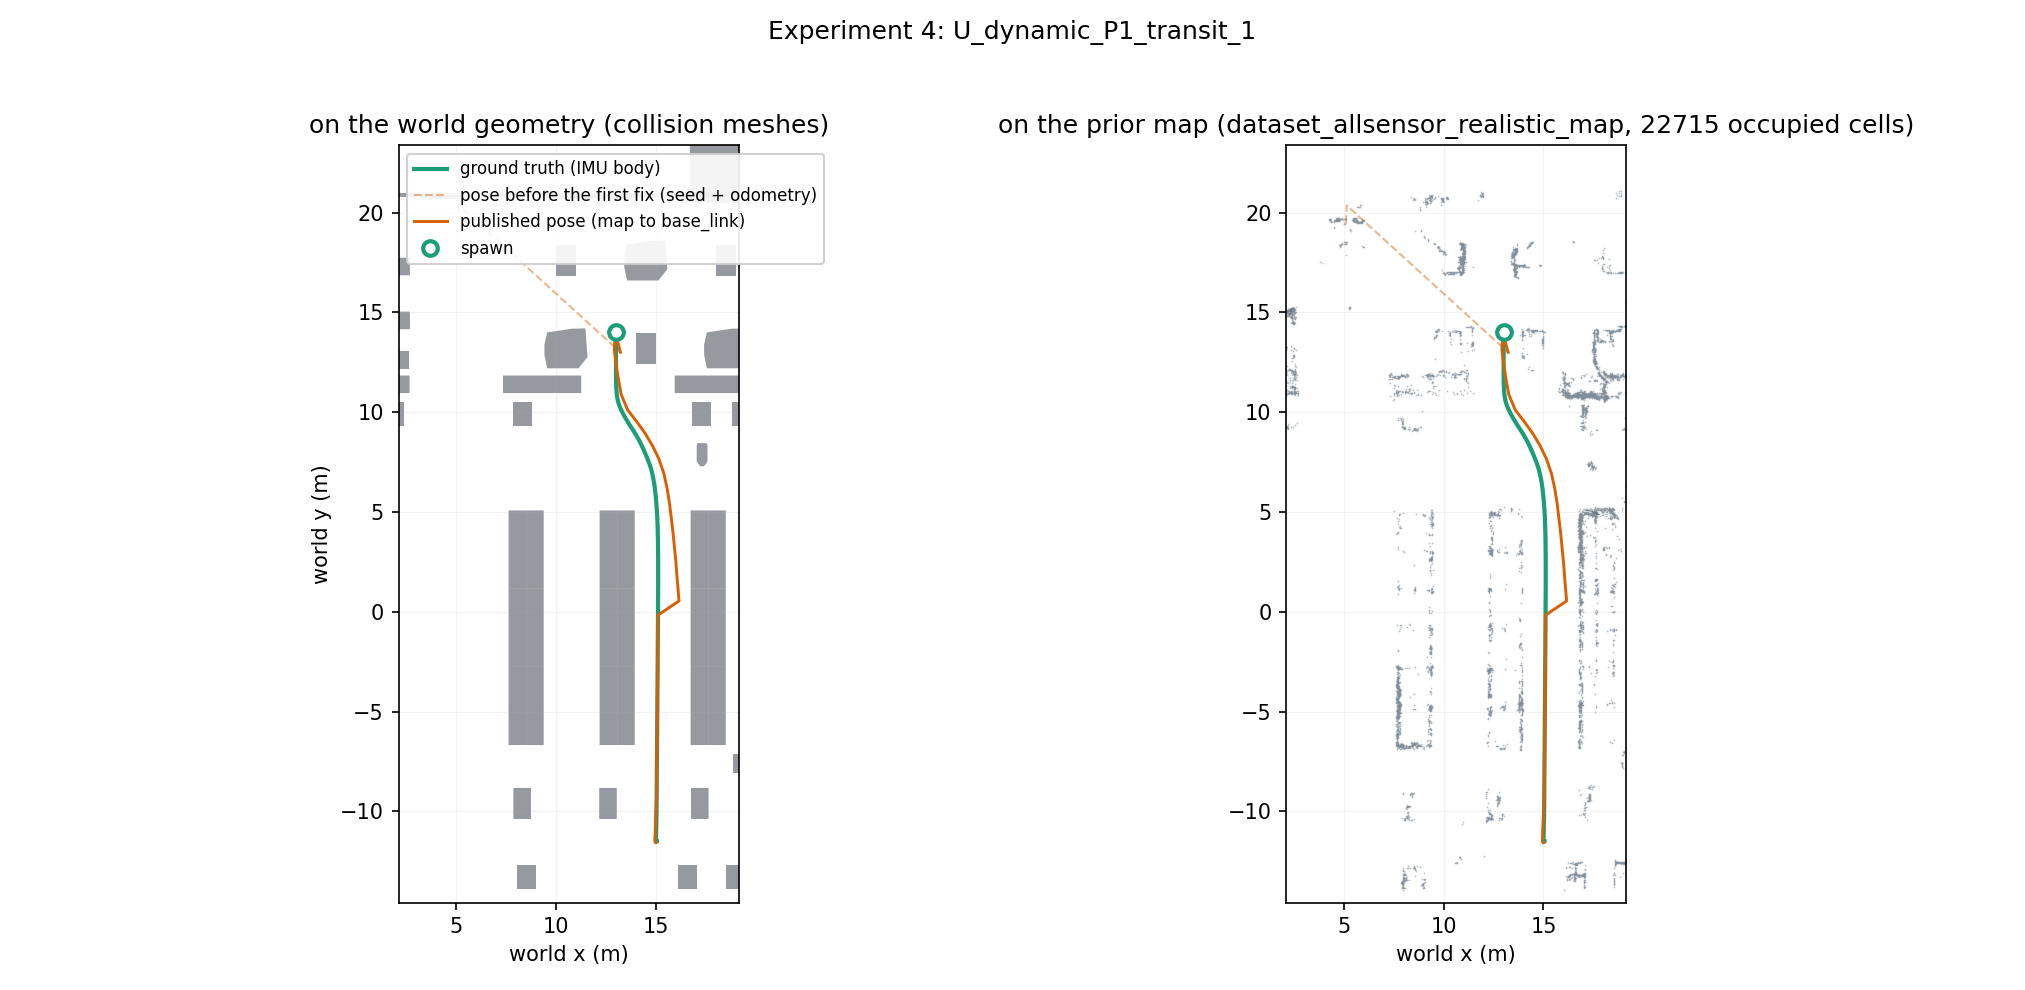
\includegraphics[width=\textwidth]{fig/exp4_path_U_dynamic_P1_transit_1.png}
  \caption{\texttt{U\_dynamic}, straight, \SI{26}{\metre}: the worst run of the
  seven on both offset (\SI{0.274}{\metre}) and scatter (\SI{0.240}{\metre}),
  and the only one with traffic. The published pose runs beside ground truth
  down the aisle rather than diverging from it, which is what a displacement
  rather than a drift looks like. Conventions as
  \cref{fig:exp4-normal}.}
  \label{fig:exp4-offset}
\end{figure}

\begin{figure}[p]
  \centering
  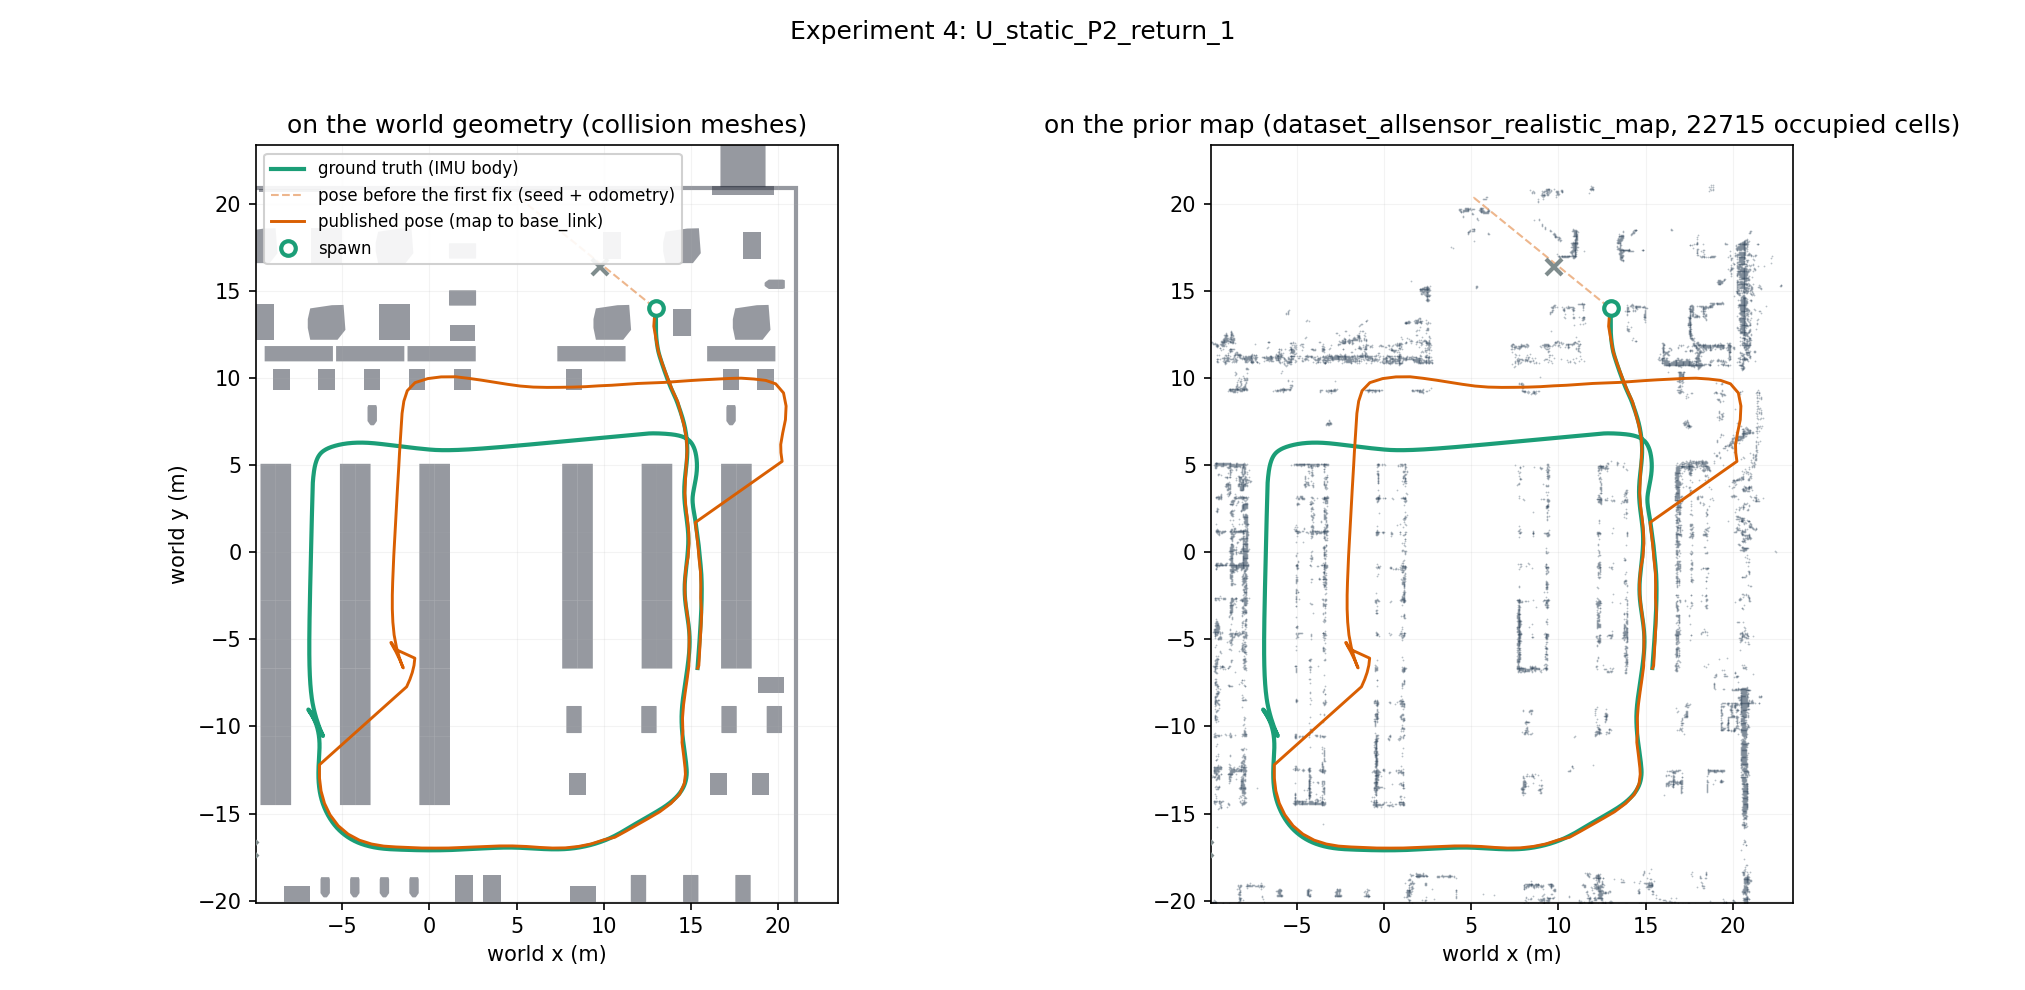
\includegraphics[width=\textwidth]{fig/exp4_path_U_static_P2_return_1.png}
  \caption{\texttt{U\_static}, approximately square, \SI{109}{\metre}: the one
  run of the seven that lost the pose. From about $y=-5$ the published pose
  leaves the aisle and cuts diagonally through three shelf rows while ground
  truth follows the aisle, which is the \SI{6.09}{\metre} second-half median of
  \cref{tab:exp4-tracking} seen directly. A pose that passes through shelving is
  wrong in a way no error statistic states as plainly. Conventions as
  \cref{fig:exp4-normal}.}
  \label{fig:exp4-diverged}
\end{figure}

\FloatBarrier
\paragraph{Heading.} Measured in the insight analysis
(\path{insights/experiment_4_insight/}) and reported here because the slot
otherwise never looks at orientation. Median heading error is below
\SI{1.2}{\degree} in all six static runs and the 95th percentile below
\SI{3.6}{\degree} in five of them, which is not a limiting quantity for a
\SI{0.6}{\metre} wheelbase in an aisle: a degree converts to
\SI{1.7}{\centi\metre} of cross-track error per metre driven. The dynamic run
is the exception, at \SI{4.85}{\degree} with a \SI{+3.35}{\degree} bias ---
four to thirteen times every static run. Traffic therefore costs heading about
tenfold where it costs position about threefold, so the position figures
understate it. Heading error does not rise with turn rate in any run.

\paragraph{Insight: the pose is as good as the map it is localising against.}
The error decomposes into a constant offset of \SIrange{0.07}{0.27}{\metre} and
scatter of \SIrange{0.04}{0.24}{\metre} about it, and almost all of it is
across the direction of travel rather than along it: once the frame error above
is removed, the along-track mean is within \SI{0.16}{\metre} of zero in every
run and changes sign between them. Cross-track error is the component that
matters for a corridor, and it is the smaller one.

The magnitude is the reading. Experiment~3 measures the graph of these same
priors as accurate to \SIrange{0.10}{0.40}{\metre} rms over the
\SIrange{365}{381}{\metre} build routes. The pose tracking that prior is
accurate to \SIrange{0.10}{0.36}{\metre}. The localiser is therefore
reproducing its map to within the map's own accuracy, and nothing in these runs
shows it doing worse than the artefact it is given. That is a bound, not a
coincidence: an estimate cannot be closer to the world than the map it is
matched against, so this slot's accuracy is \emph{map-limited rather than
estimator-limited}, and the improvement to chase is a better prior rather than a
better filter.

\flag{The previous revision drew a stronger conclusion from the same data ---
that the offset was route-dependent, \SIrange{0.32}{0.59}{\metre} on a single
aisle against \SIrange{0.02}{0.14}{\metre} over the building, and matched
Experiment~3's half-metre wall displacement. That pattern was the frame error,
which is larger on a straight run where the heading barely changes. It does not
survive the correction and is withdrawn.}

\paragraph{Insight: the initialisation transient damages both layers.}
Experiment~3 attributes the blocking false obstacles of three of the four
realistic maps to phantom cells laid by the first five graph nodes
(\SIrange{63}{96}{\percent} of them), and names discarding those cells, or
starting the map after the inertial transient has settled, as the one
correction its data predict would help. The same transient was found
independently in this slot, one layer up: the front end's orientation is
unstable for about a second after it starts, and a back end that accepts a fix
during that window latches a correction \SIrange{73}{76}{\degree} wrong and
holds it for roughly \SI{16}{\second}. Holding the back end back for
\SI{5}{\second} removed it, confirmed over three runs by the collapse of the
largest correction yaw from \SIrange{110}{177}{\degree} to \SI{25}{\degree}.
Neither \repo{wait_for_imu_init} nor the pose gate's \repo{init_ignore_s}
prevents it: the first tests inertial validity, which is already true through
the unstable window, and the second only withholds the pose from Nav2 after the
correction has been formed. One transient, two symptoms, and the same
prescription in both places --- do not consume the first second.

\paragraph{Excursions, and that every one of them ended.} Two runs left the
map for tens of seconds. The U static square route was over a metre from ground
truth for \SI{36}{\second}, reaching \SI{6.8}{\metre}, and the U static
figure-of-eight for \SI{23.5}{\second}, reaching \SI{4.0}{\metre}. Both then
recovered: the last tenth of each run sits at \SI{0.106}{\metre} and
\SI{0.120}{\metre}. The U dynamic run had a shorter one, \SI{2.5}{\second}.
The four remaining runs never crossed a metre at all.
\Cref{fig:exp4-summary} shows all seven on one axis, and the two long
excursions as the flat shelves they are --- the pose does not drift away and
come back, it steps off, holds a wrong place, and steps back when a correct fix
lands.

The two are not the same fault, which the corrections show and the error curves
do not. On the figure-of-eight the correction's yaw moves from
\SI{-0.5}{\degree} to \SI{+11.0}{\degree} and back, heading error inside the
stretch is \SI{11.0}{\degree} against \SI{0.4}{\degree} outside it, and
heading and position error correlate at $r=0.97$: the robot was placed facing
the wrong way, and driving converted the angle into displacement. On the square
the correction's yaw barely moves while its translation shifts over
\SI{5}{\metre}: the robot was placed in the wrong aisle at the right heading.
These are the warehouse's two symmetries, the aisle pitch and the orientation of
a bay, and a defence aimed at one does not catch the other --- the same split
the November acceptance sweep found among individual rejected fixes.

\flag{Two earlier claims are withdrawn. The square route was described as
having ``lost the pose'' and ``not recovered before the run ended''; it
recovered \SI{9}{\second} before the end, to \SI{0.011}{\metre} on the final
sample. The figure-of-eight was reported as clean, because its excursion sits
inside the first half and a half-by-half median hid it. Both errors came from
summarising with medians and a maximum and no measure of duration, which is why
the table now carries one.}

Availability is the weaker column. The I static straight run carried no
information for \SI{15.8}{\percent} of its poses and the U dynamic run for
\SI{10.3}{\percent}, against a criterion of \SI{10}{\percent}. Accuracy in both
was ordinary when a fix existed, so the difficulty is holding the fix rather
than obtaining one.

\paragraph{Insight: over these distances the prior supplies a datum, not
accuracy.} \flag{This narrows the objective stated above, and is the claim the
data support.} Unaided ORB-SLAM3, rigidly aligned onto ground truth, drifts by a
median of \SIrange{0.045}{0.345}{\metre} over these \SIrange{21}{152}{\metre}
routes, never exceeds \SI{0.76}{\metre} at any instant, and ends each run
between \SI{0.03}{\metre} and \SI{0.60}{\metre} from truth. Run by run the
medians split three to three with one tie against the localised pose, so
localising on the map does not improve local accuracy here --- and it introduces
excursions an order of magnitude larger than the front end produced alone,
\SI{6.80}{\metre} and \SI{3.99}{\metre} against a front-end worst of
\SI{0.76}{\metre}.

What the prior does supply is the thing that comparison gives the front end for
free: an absolute, repeatable datum in a frame that outlives the run, which is
what lets a goal in map coordinates mean the same place twice. Over these route
lengths that is the whole of its contribution, bought at two multi-second
excursions in seven runs. The prediction worth testing is that it begins to pay
for itself in accuracy where front-end drift exceeds the localisation error,
beyond \SI{152}{\metre}; the \SIrange{365}{381}{\metre} mapping routes should
already reach that.

\paragraph{Traffic.} The one dynamic run is the worst of the seven on both
offset (\SI{0.588}{\metre}) and scatter (\SI{0.247}{\metre}, about double the
static runs) and sat unlocalised \SI{10.3}{\percent} of the time. One run
decides nothing, but it points the same way as Experiment~1's finding that
traffic degrades the estimate without breaking tracking.

\paragraph{What these data cannot answer.} Every cell is a single run, and the
acceptance sweep of 11--12 November established that this stack's run-to-run
spread over identical settings is as wide as most differences between settings,
so no comparison between worlds, layouts or routes in
\cref{tab:exp4-tracking} is evidence. The routes were driven by hand and
differ in shape and length, so route is a confound rather than a factor. No
goal was commanded, so nothing here speaks to planning, to the false-obstacle
question that motivates the experiment, or to recovery behaviour. One dynamic
world is sampled and one is not.

\paragraph{Next action.} Collect the dynamic worlds and reps 2 and 3 of every
cell, then run the goal set with \texttt{--run} so the goal-reaching rules above
can be applied. The narrow question still outstanding is Experiment~3's: does
the \SIrange{3.8}{10.2}{\percent} false-obstacle rate block a route, or does the
planner drive around it.


\FloatBarrier
\section{Every run}
\label{sec:exp4-allruns}

The three runs not drawn above, for completeness; conventions as
\cref{fig:exp4-normal}.

\begin{figure}[p]
  \centering
  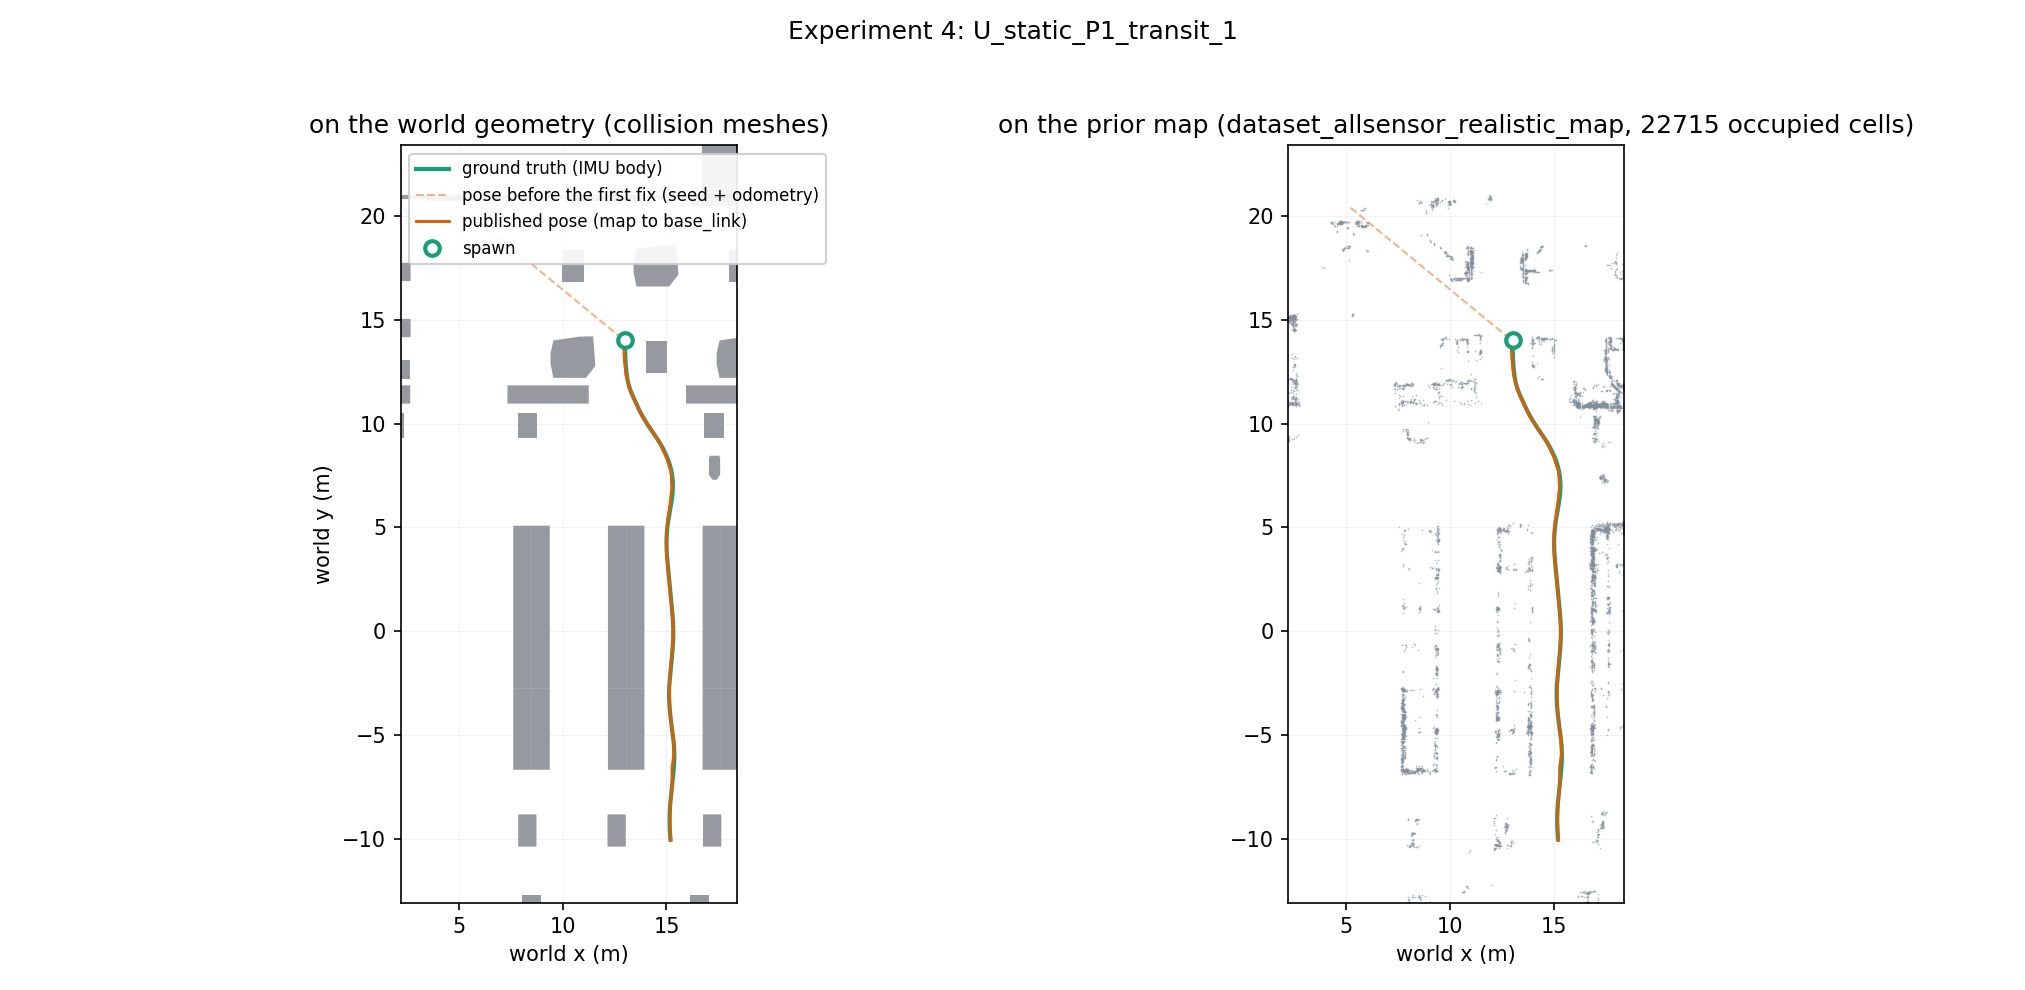
\includegraphics[width=0.92\textwidth]{fig/exp4_path_U_static_P1_transit_1.png}
  \caption{\texttt{U\_static}, straight, \SI{24.6}{\metre}. The two tracks are
  indistinguishable at this scale, which is the point: the median error is
  \SI{0.162}{\metre} and the run never crossed a metre. It is also the figure
  that exposed the lever-arm error --- a \SI{0.47}{\metre} offset was being
  reported for a run whose tracks visibly coincide, which is only possible if
  the offset lies along the direction of travel, where a path plot cannot show
  it.}
  \label{fig:exp4-u-straight}
\end{figure}

\begin{figure}[p]
  \centering
  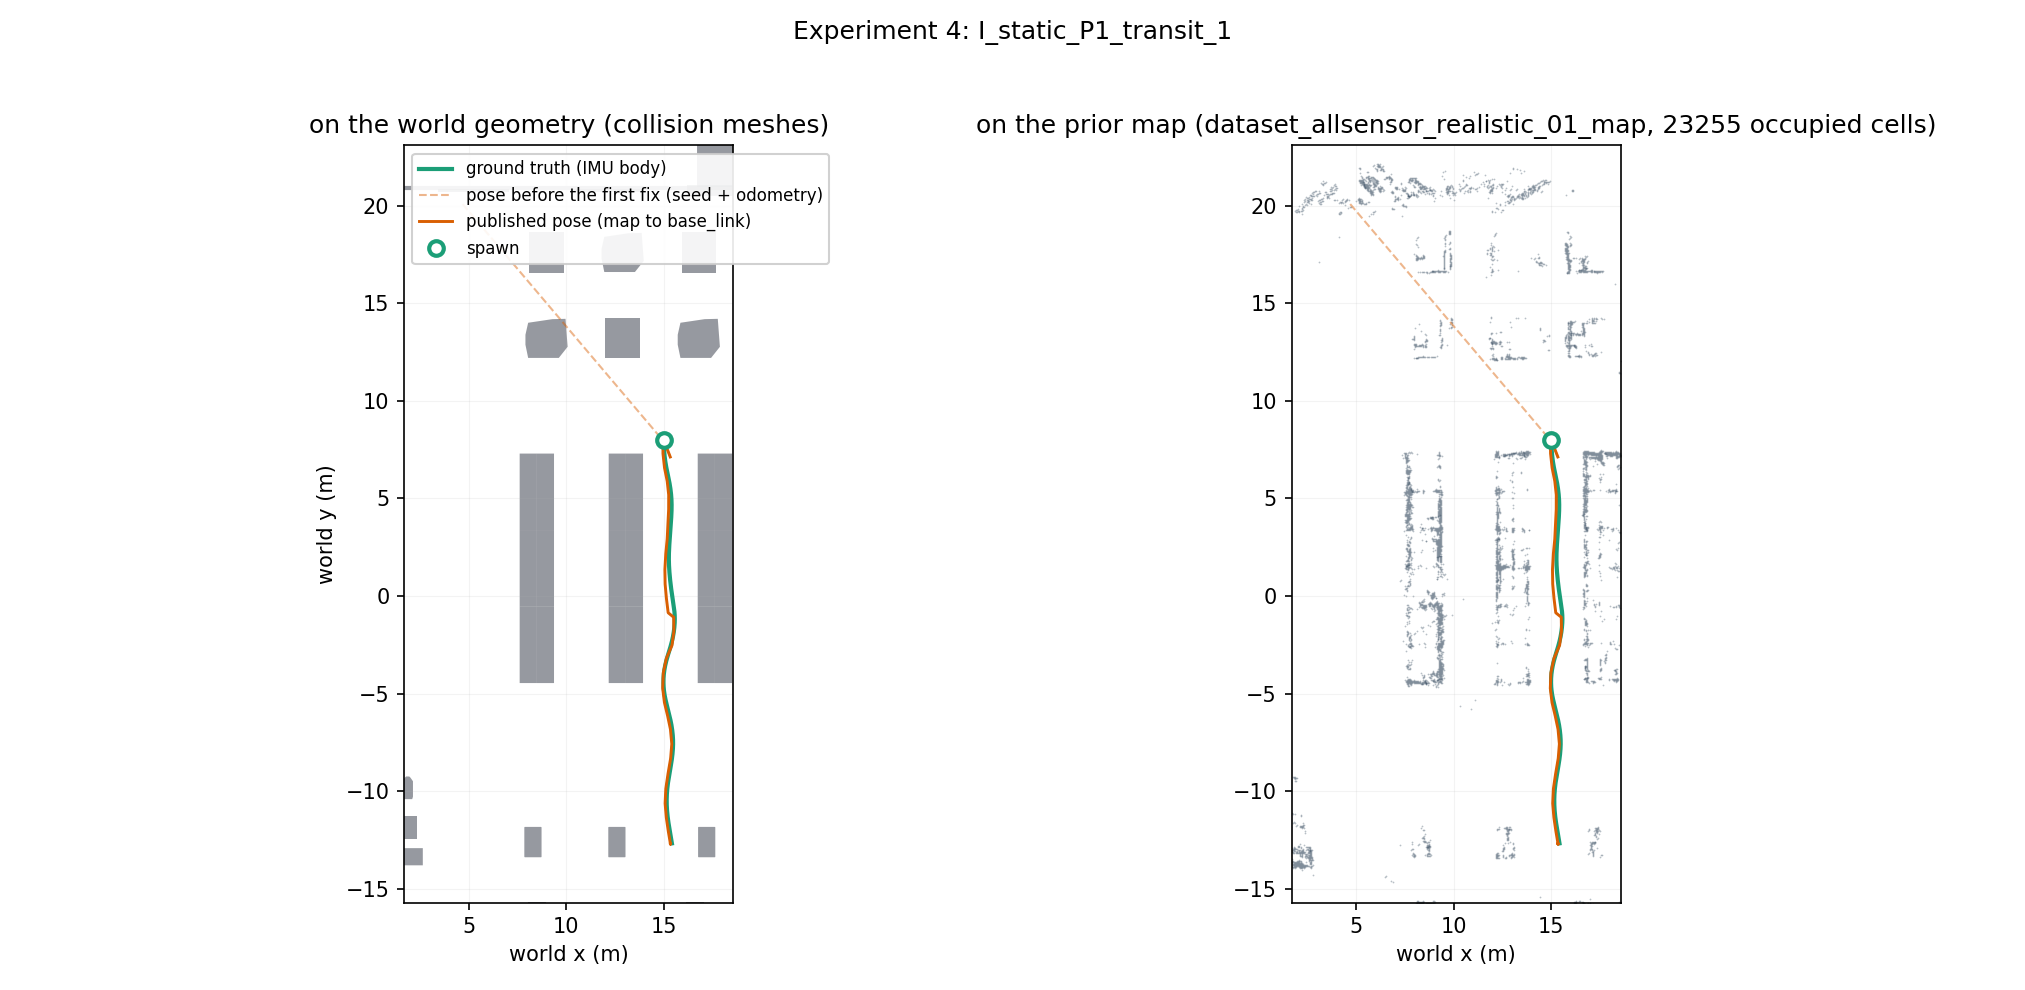
\includegraphics[width=0.92\textwidth]{fig/exp4_path_I_static_P1_transit_1.png}
  \caption{\texttt{I\_static}, straight, \SI{20.9}{\metre}: the most accurate
  run of the seven by median (\SI{0.097}{\metre}) and the least available, with
  \SI{15.8}{\percent} of its poses carrying no information. Accuracy and
  availability are separate properties and this run holds the extreme of both.}
  \label{fig:exp4-i-straight}
\end{figure}

\begin{figure}[p]
  \centering
  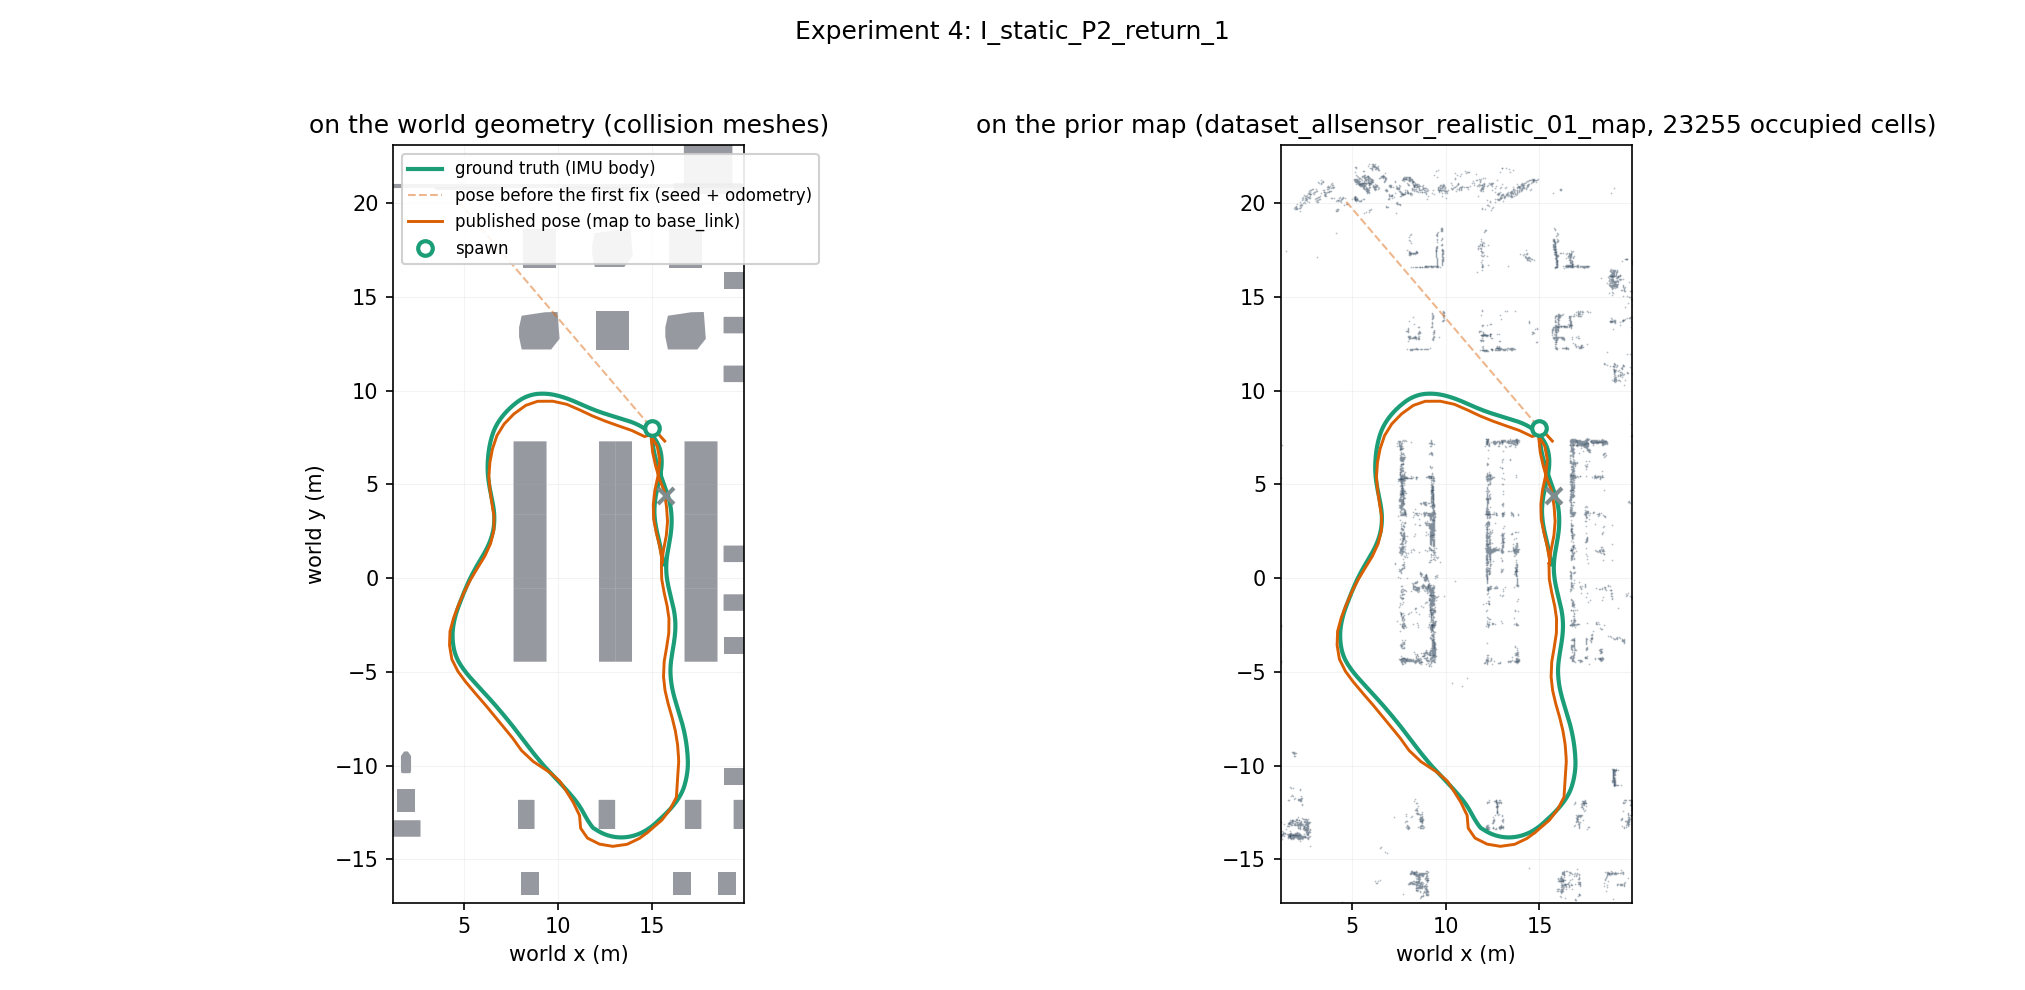
\includegraphics[width=0.92\textwidth]{fig/exp4_path_I_static_P2_return_1.png}
  \caption{\texttt{I\_static}, approximately square, \SI{66.8}{\metre}: the
  largest median of the seven at \SI{0.361}{\metre}, with no excursion over a
  metre and an offset of \SI{0.204}{\metre}. A consistently displaced pose
  rather than an unstable one, and the case that sets the upper end of the
  \SIrange{0.10}{0.36}{\metre} range.}
  \label{fig:exp4-i-square}
\end{figure}

% =====================================================================
\FloatBarrier
\section{Real robot}
\label{sec:exp4-real}

\slotstatus{planned}{No real-robot navigation run has been made, and the real
rig has no map to navigate on: the dense-map slot of the real-robot slot of
Experiment~3 is itself planned, because no RTAB-Map database has been built
from real imagery and no reference geometry of the site exists to score one
against.}

\paragraph{Objective.} As in simulation, on the real rig.

\paragraph{Next action.} Blocked behind the real-robot half of Experiment~3: a
map must exist before navigation on it can be scored. The \SI{5}{\second} back
end hold that works in simulation is a fixed guess at the length of the front
end's unstable window and should not be carried to the rig unchanged; the
transferable form is an orientation-stability condition in the front end
itself.

\end{document}
